\chapter{Design and Realization of Static Action Discovery}

This section provides an outline of the methods and materials used to create, benchmark, and assess a new routing mechanism. Initially, we'll discuss the benchmark application that employs the existing routing solution by Microsoft, serving as the basis for our study. Subsequently, we'll explore the modified application, highlighting its differences from the benchmark. The implementation details will be further addressed in the next chapter. Lastly, we'll define the testing metrics, scenarios, and environments used and explain how we ensured the reproducibility of our results.


\section{Characteristics of the Benchmark Application}

This subsection delves into the specifics of the benchmark application used in this research, developed as an ASP.NET Core Web API. A key characteristic of this application, and indeed a cornerstone of its design, is the usage of reflection-based routing discovery. While widely employed, this mechanism inspects every class within the project and loaded assemblies. As the codebase grows, the efficiency of this approach decreases, presenting a challenge that our new implementation seeks to overcome.

The benchmark application is constructed with simplicity in mind, serving as a baseline for evaluating our novel routing implementation. Yet, despite its simplicity, it effectively mimics an enterprise application, which forms the intended user base of our tool. It consists of 10,000 controllers with varying complexities, each housing a different number of exposed actions and diverse routing attributes. This intricate setup is designed to simulate scenarios commonly encountered in a real-world Web API.

A point of significance is that the benchmark application, like our modified app, is written as part of the official ASP.NET Core repository. This choice is motivated by our implementation requirements, which involve modifications to the existing framework alongside the addition of new features. Such changes couldn't have been achieved through an external NuGet package, necessitating our presence within the official repository. We've ensured a consistent environment for both apps to ensure the most accurate comparisons, thus minimizing potential interference from variables like differing .NET SDKs.

The benchmark application is streamlined, focusing on the core functionalities of a Web API to maximize testing accuracy. By excluding additional features such as authentication or Cross-Origin Resource Sharing (CORS), we eliminate the potential overhead that could equally affect both the standard and modified applications, thereby enhancing the precision of our tests.

Lastly, we've designed the benchmark setup with a keen focus on reproducibility. The comprehensive description of the application's structure and configurations in this section offers a path for others to replicate these tests and reproduce our results. This ensures that the results we gather are not biased due to extraneous variables, thereby improving the repeatability and reliability of our tests.

\section{Enhancing Action Discovery: A New Perspective}

As we delve into the intricacies of static action discovery, it's essential to grasp how this approach reshapes the traditional application structure. The following sections unravel this transformative process, beginning with an exploration of action discovery and its significance in routing. We then introduce the concept of static action discovery, providing a comprehensive view of its development. By journeying through these stages, we aim to provide a solid understanding of this new structure and its potential performance benefits.

\subsection{Understanding Action Discovery and Its Role in Routing}

ASP.NET Core is a web framework designed to process various user requests. Based on incoming URLs, HTTP Methods, and Bodies, these requests are directed toward specific actions. Actions can be routed in two distinct ways: via conventional routes, which are manually defined during the start-up phase, or via attribute-based routing, where routes are defined through annotations on the controllers and their actions.

Figure \ref{fig:conventional-routing} depicts a conventional routing approach. In this example, a route named default is created, generating a pattern against which routes are matched. The route path is tokenized into controllers, actions, and parameters. The extracted tokens correspond to the components of an application. However, manually declaring all routes is time-consuming and error-prone, as routes must always be synchronized with the controllers.

\begin{figure}[H]
\centering
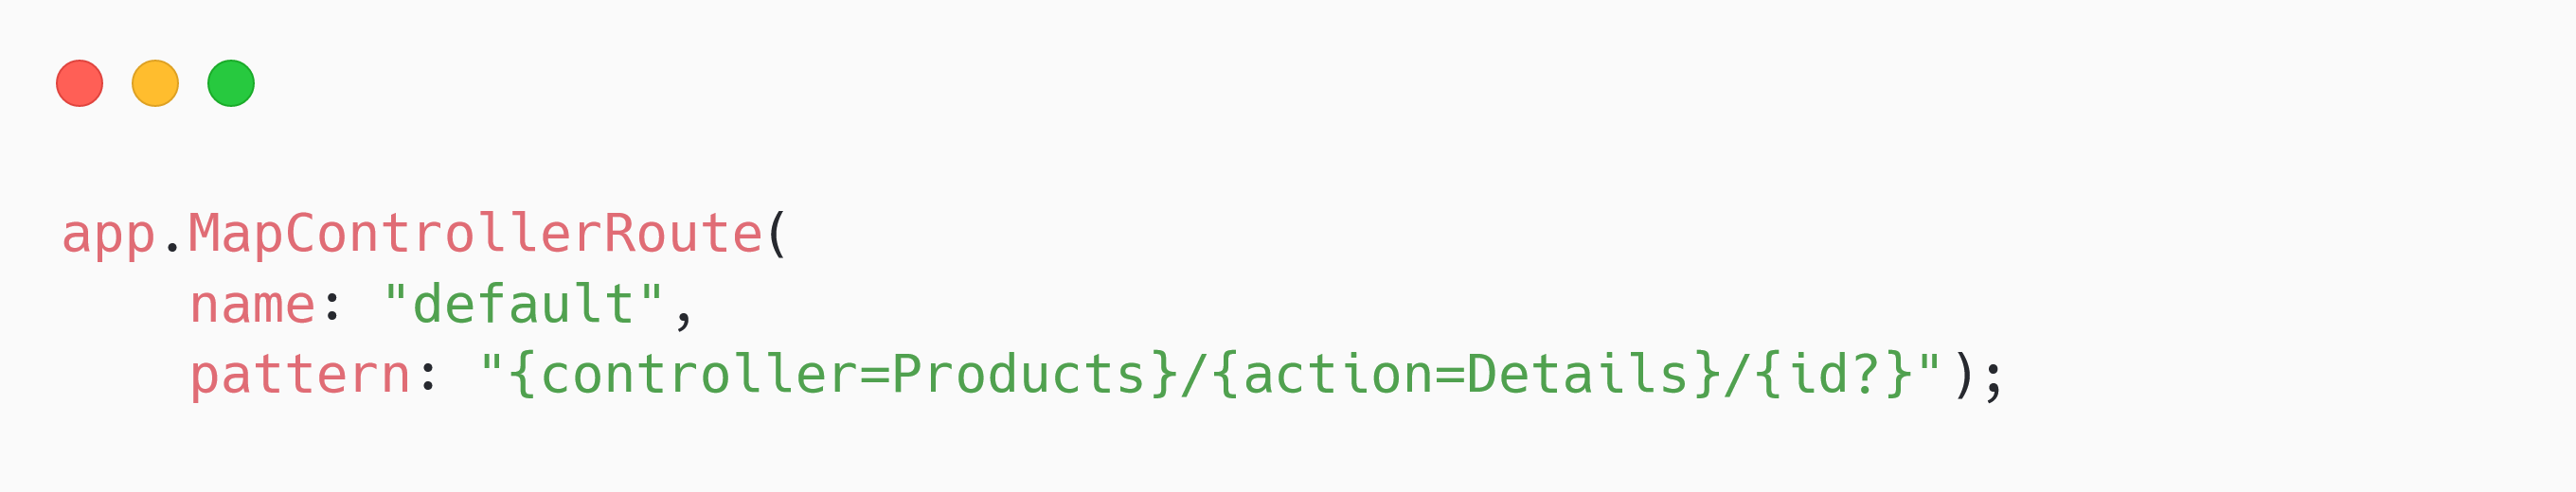
\includegraphics[width=0.8\textwidth]{graphics/conventional-routing.png}
\caption{An example of conventional routing in ASP.NET Core}
\label{fig:conventional-routing}
\end{figure}

To overcome the limitations of conventional routing, attribute-based routing is often used. Here, routes are declared on the controllers directly via attributes, ensuring synchronization between the routes and the controllers and eliminating manual intervention. Figure \ref{fig:attribute-routing} showcases a similar controller as depicted in Figure \ref{fig:conventional-routing}, but with attribute-based routing.

\begin{figure}[H]
\centering
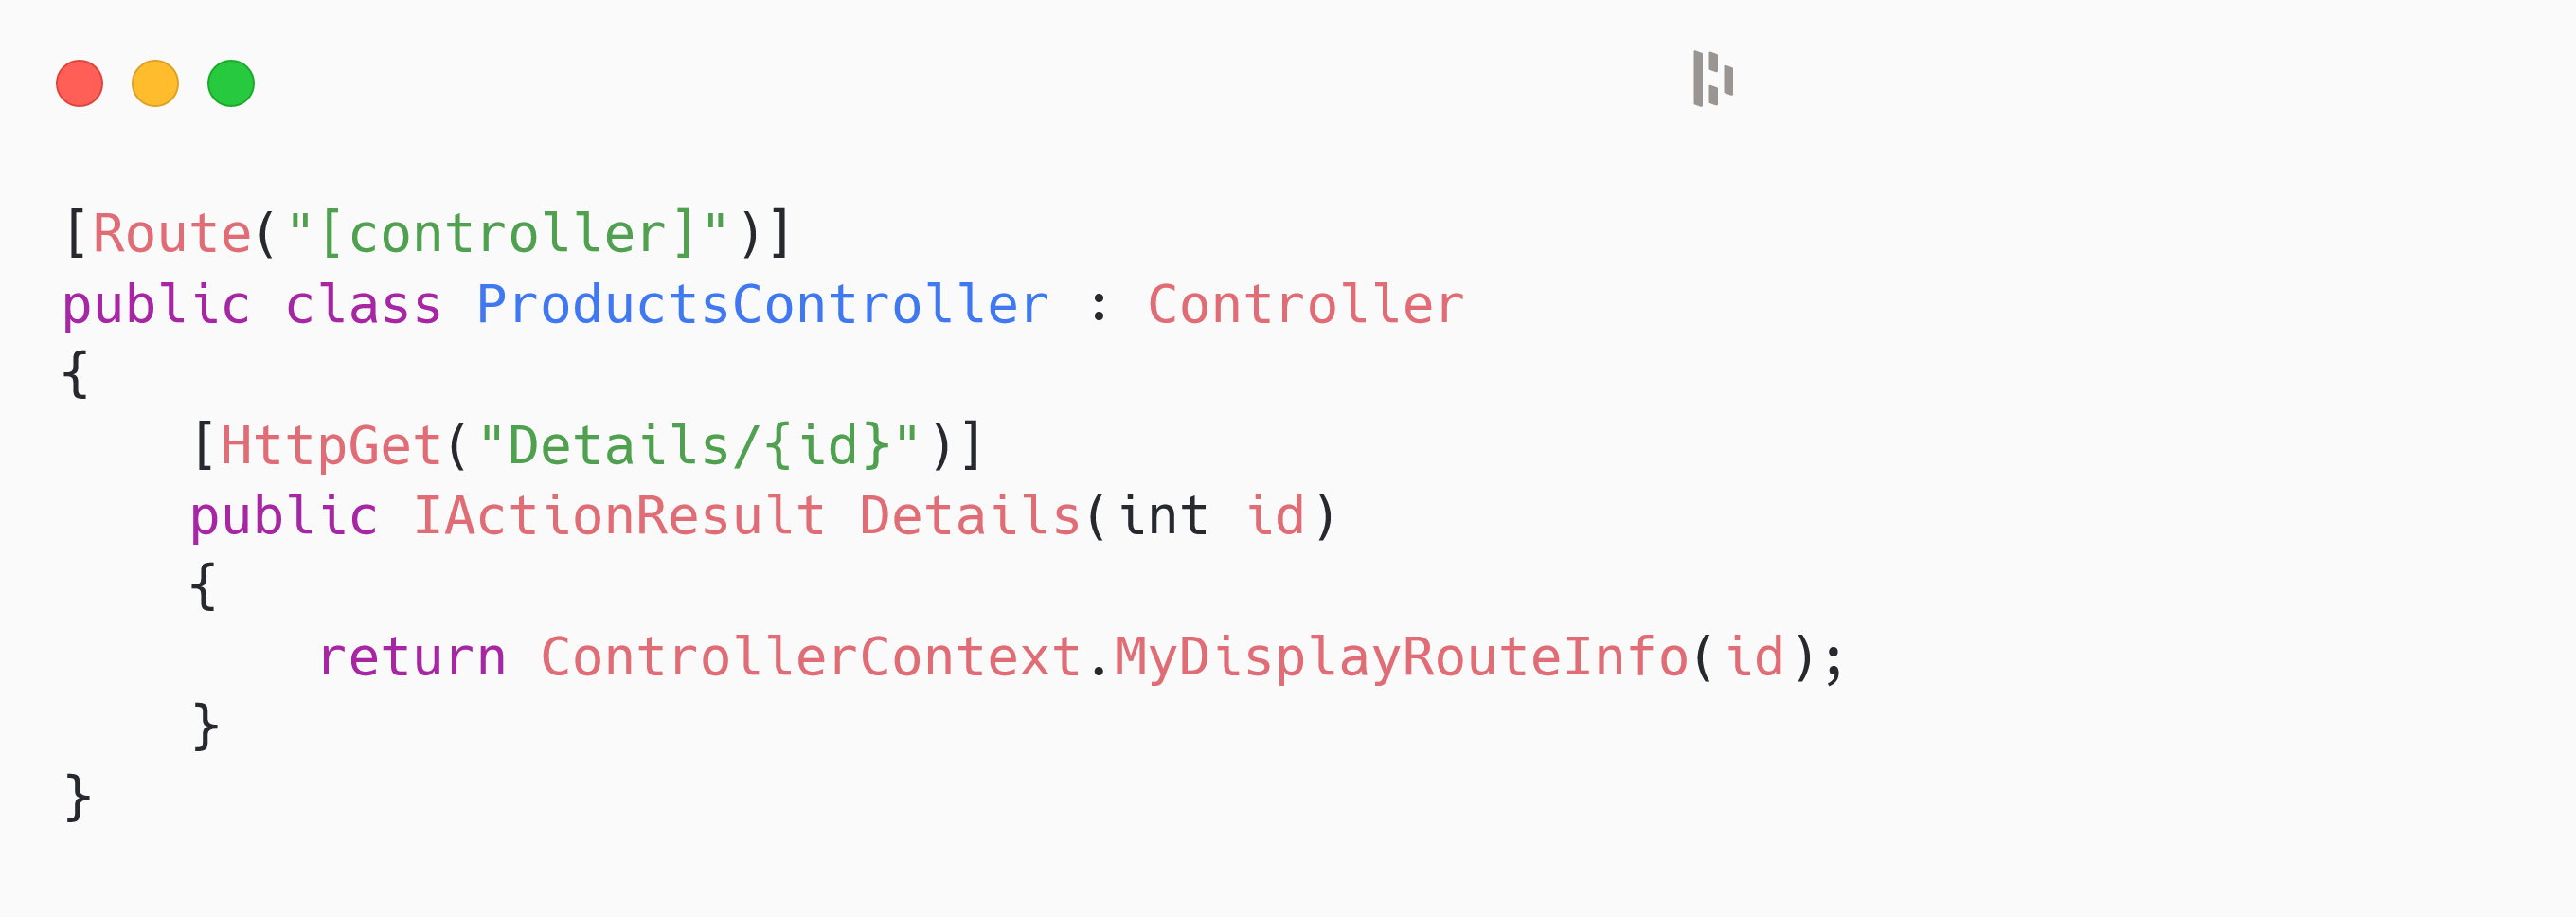
\includegraphics[width=0.8\textwidth]{graphics/attribute-routing.png}
\caption{An example of attribute-based routing in ASP.NET Core}
\label{fig:attribute-routing}
\end{figure}

While attribute-based routing offers an improvement over conventional routing, both approaches have a common drawback: they require a thorough knowledge of all controllers and actions for the routing mechanism. Therefore, during the application's start-up phase, a process known as 'action discovery' is initiated, which examines the entire code base to identify all controllers and their corresponding actions.

During application start-up, this action discovery process is launched by calling the \\"app.MapControllers()" method. The action discovery involves two significant services registered by the MVC framework. The first service analyzes every file in all referenced assemblies, including third-party tools like Swagger, identifying potential controllers. These identified controllers are then analyzed by a second service, which uses reflection to extract all the routing information.

Although this process is thorough, it can be resource-intensive for larger applications, resulting in performance overhead each time the application is started. Our new tool aims to mitigate this overhead by generating static code at compile time without reflection, optimizing the action discovery process. This tool and its workings will be discussed in detail in the next section.

\subsection{Introducing the Static Action Discovery}

In our approach, we rely on incremental source generators. These tools come into play during the application's build process, producing additional source code that becomes part of the final executable. Crucially, source generators are designed for efficiency, executing only when a change in the output is detected. The nitty-gritty details of this process will be delved into in a separate chapter devoted to implementation details.

Our source generator, during its operation, creates several key files. It spawns a service extension, which allows adding the required MVC framework without needing dynamic action discovery. Furthermore, a unique static action discovery service is created for every controller found within the project.

Let's compare this to the conventional way of integrating the MVC framework into an ASP.NET Core application. This process is illustrated in Figure \ref{fig:dynamic-action-discovery}.

\begin{figure}[H]
\centering
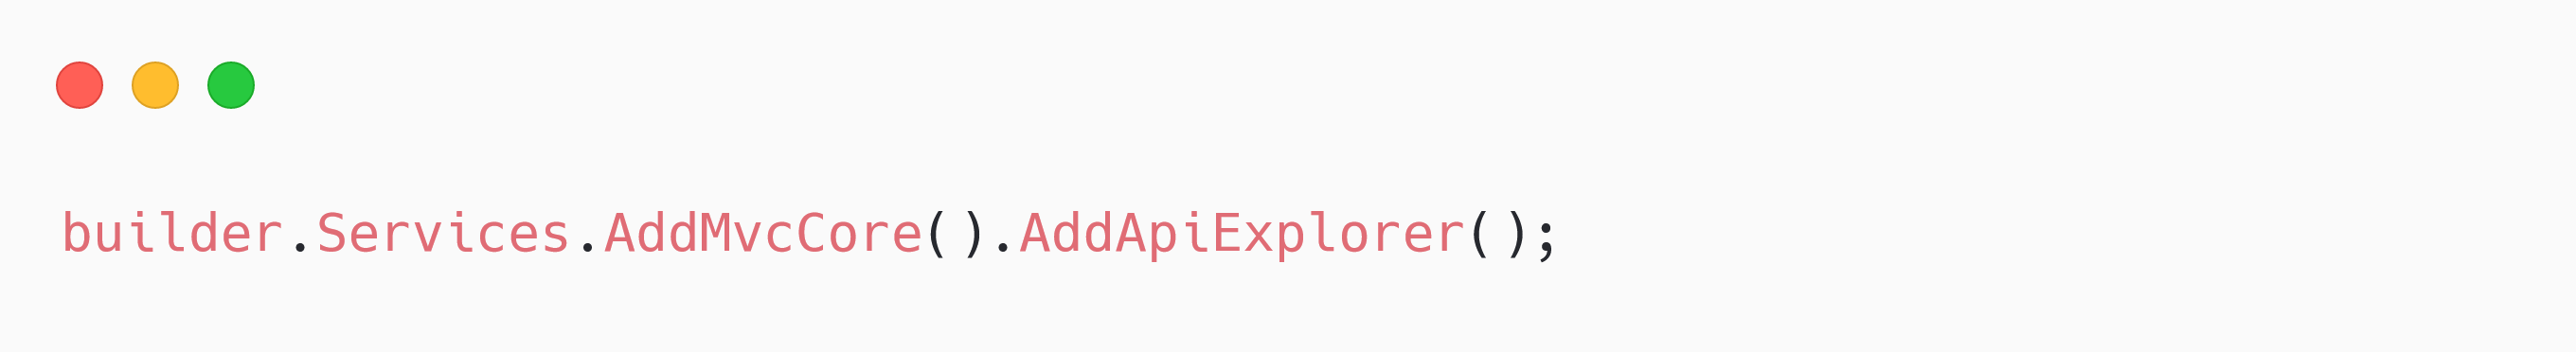
\includegraphics[width=0.8\textwidth]{graphics/dynamic-action-discovery.png}
\caption{Adding the MVC Framework in a traditional ASP.NET Core Application}
\label{fig:dynamic-action-discovery}
\end{figure}

Moving on to our proposed approach, we simplify the process as shown in Figure \ref{fig:static-action-discovery}.

\begin{figure}[H]
\centering
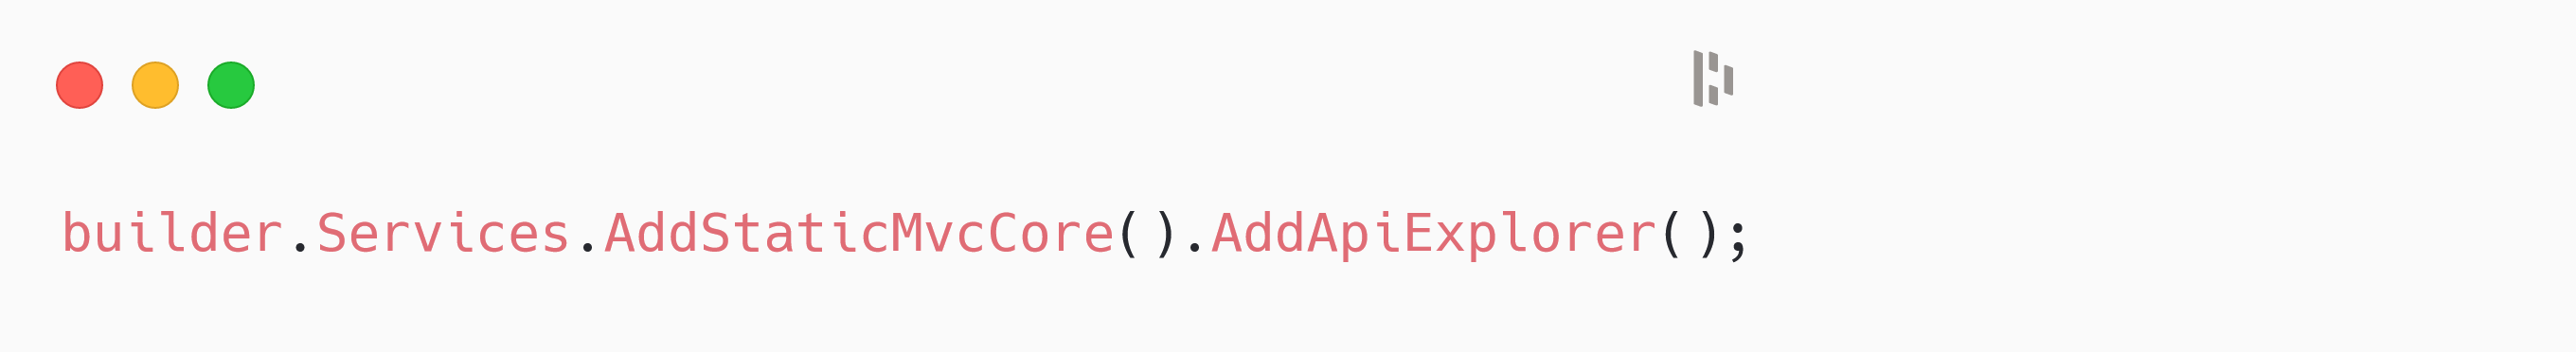
\includegraphics[width=0.8\textwidth]{graphics/static-action-discovery.png}
\caption{Adding the MVC Framework using our new approach}
\label{fig:static-action-discovery}
\end{figure}

While the methods appear virtually identical, it's worth noting that the AddStaticMvcCore method is neither stored in any Git repository nor is it part of the project where the source generator is defined. Instead, it is generated by the project that consumes the source generator, allowing the method to be custom-tailored to each application for potential action discovery optimization.

The AddStaticMvcCore method registers the MVC framework and an action discovery service for every controller in the project under development. The services harbor all metadata the routing mechanism requires to map endpoints to the controllers.

A significant challenge arises due to source generators running as part of the compilation process, making reflection an impractical tool. Reflection, used in dynamic action discovery, inspects controllers and reads all the attributes applied to the controllers and actions. However, reflection is unusable since the code is not ready to run at the point of the compilation process. Instead, we use the Roslyn API to inspect the Syntax Tree and the Semantic Model of the controllers.

The Syntax Tree and Semantic Model allow us to extract the necessary information in a manner similar to reflection but without running the code. However, this means we can only extract information that can be parsed deterministically at compile time, excluding the values of properties or execution of code snippets.

Fortunately, the static action discovery relies on Attributes, the parameters of which must be compile-time constants and can be evaluated. The challenge arises when these attributes use properties that don't fall under the same restriction. Figure \ref{fig:custom-property} shows an example of such an attribute.

\begin{figure}[H]
\centering
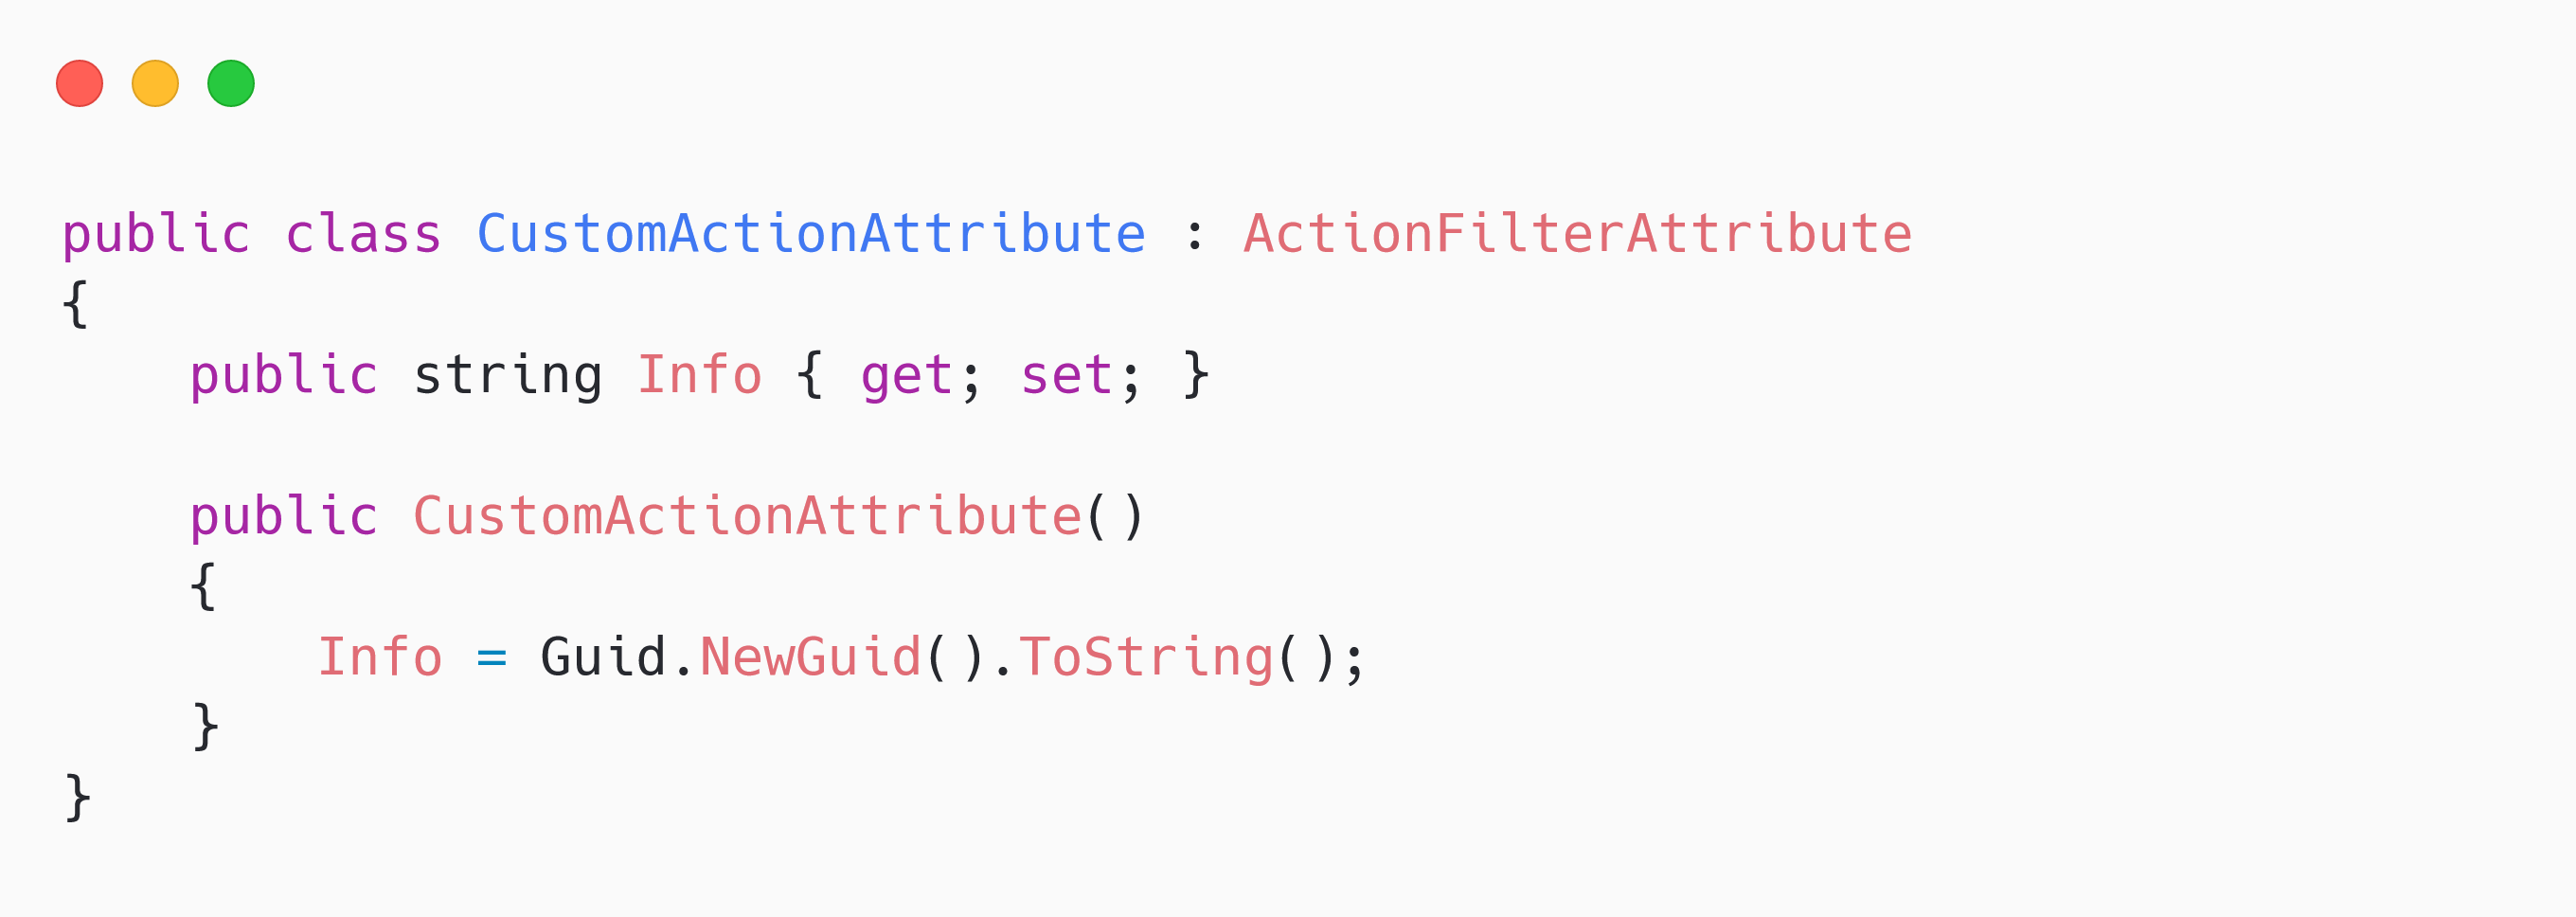
\includegraphics[width=0.8\textwidth]{graphics/custom-property.png}
\caption{Example of a Custom Attribute with Non-deterministic Property Value}
\label{fig:custom-property}
\end{figure}

Upon extracting the required attributes, they are stored as static source code added to the application model executed during the startup. The routing mechanism receives the same application model it would with dynamic action discovery, ensuring seamless integration.

\subsection{Project Structure Options and Decisions}

When developing a source generator for static action discovery, two primary strategies emerge: creating a standalone repository referencing the ASP.NET Core SDK, or modifying the official ASP.NET Core repository directly. Each of these approaches carries its own set of advantages and disadvantages.

Creating a new repository provides the advantage of an easy and straightforward setup process. However, it brings along a significant drawback. It doesn't allow for modifying the existing implementation of the MVC framework, which is crucial for our project. The need to remove the dynamic action discovery services implies that after integrating the MVC framework, one would have to loop over all registered services in the Dependency Injection container and discard those related to dynamic action discovery. This approach is far from clean, incurs an avoidable performance overhead, and contradicts our project's main goal - minimizing performance overhead. Leaving the dynamic action discovery services as they are would lead to both static and dynamic action discoveries running simultaneously. This would undeniably increase the startup time and potentially cause parts of the application to malfunction due to the ambiguity of endpoints, created twice in this scenario.

In contrast, modifying the official ASP.NET Core repository provides a more elegant solution. It allows for the MVC framework's modification to exclude dynamic action discovery when static action discovery is in use. Importantly, it enables us to include the generators as part of the SDK, enhancing the end user's ease of use. The only requirement for utilizing the generated static action discovery is referencing the generator project, informing the compiler about its existence, and triggering the generation process during builds.

In addition to these points, using the official repository has a few more benefits. It provides direct access to ASP.NET Core's latest updates and features. Also, modifications made in the official repository contribute directly to the ASP.NET Core community, enhancing the open-source ecosystem's vitality and productivity.

\subsection{Approaches to Static Code Generation}

Once the overarching project structure has been settled, the next step is creating the static code representing the application model. For this task, we have two viable options at our disposal: building a string representation of the source code or employing SyntaxFactory.

String representation, although straightforward, tends to be error-prone and challenging to maintain. On the other hand, SyntaxFactory, while verbose and having a slight overhead, offers a more reliable approach. It facilitates the creation of individual statements, allows for easy renaming of variables, and ensures that the resulting source code is syntactically correct and automatically formatted. Despite its overhead, the numerous benefits provided by SyntaxFactory greatly outweigh its drawbacks, making it our preferred choice for this task. 

Figure \ref{fig:syntax-factory} depicts an example of SyntaxFactory's utilization. It demonstrates the creation of a simple method, accepting a string parameter and returning a new ControllerModel. It's important to note that the actual method body isn't included within this segment and will be integrated into subsequent portions of the code. This example illustrates the flexibility offered by SyntaxFactory, enabling us to modularize the code generation process effectively.

\begin{figure}[H]
\centering
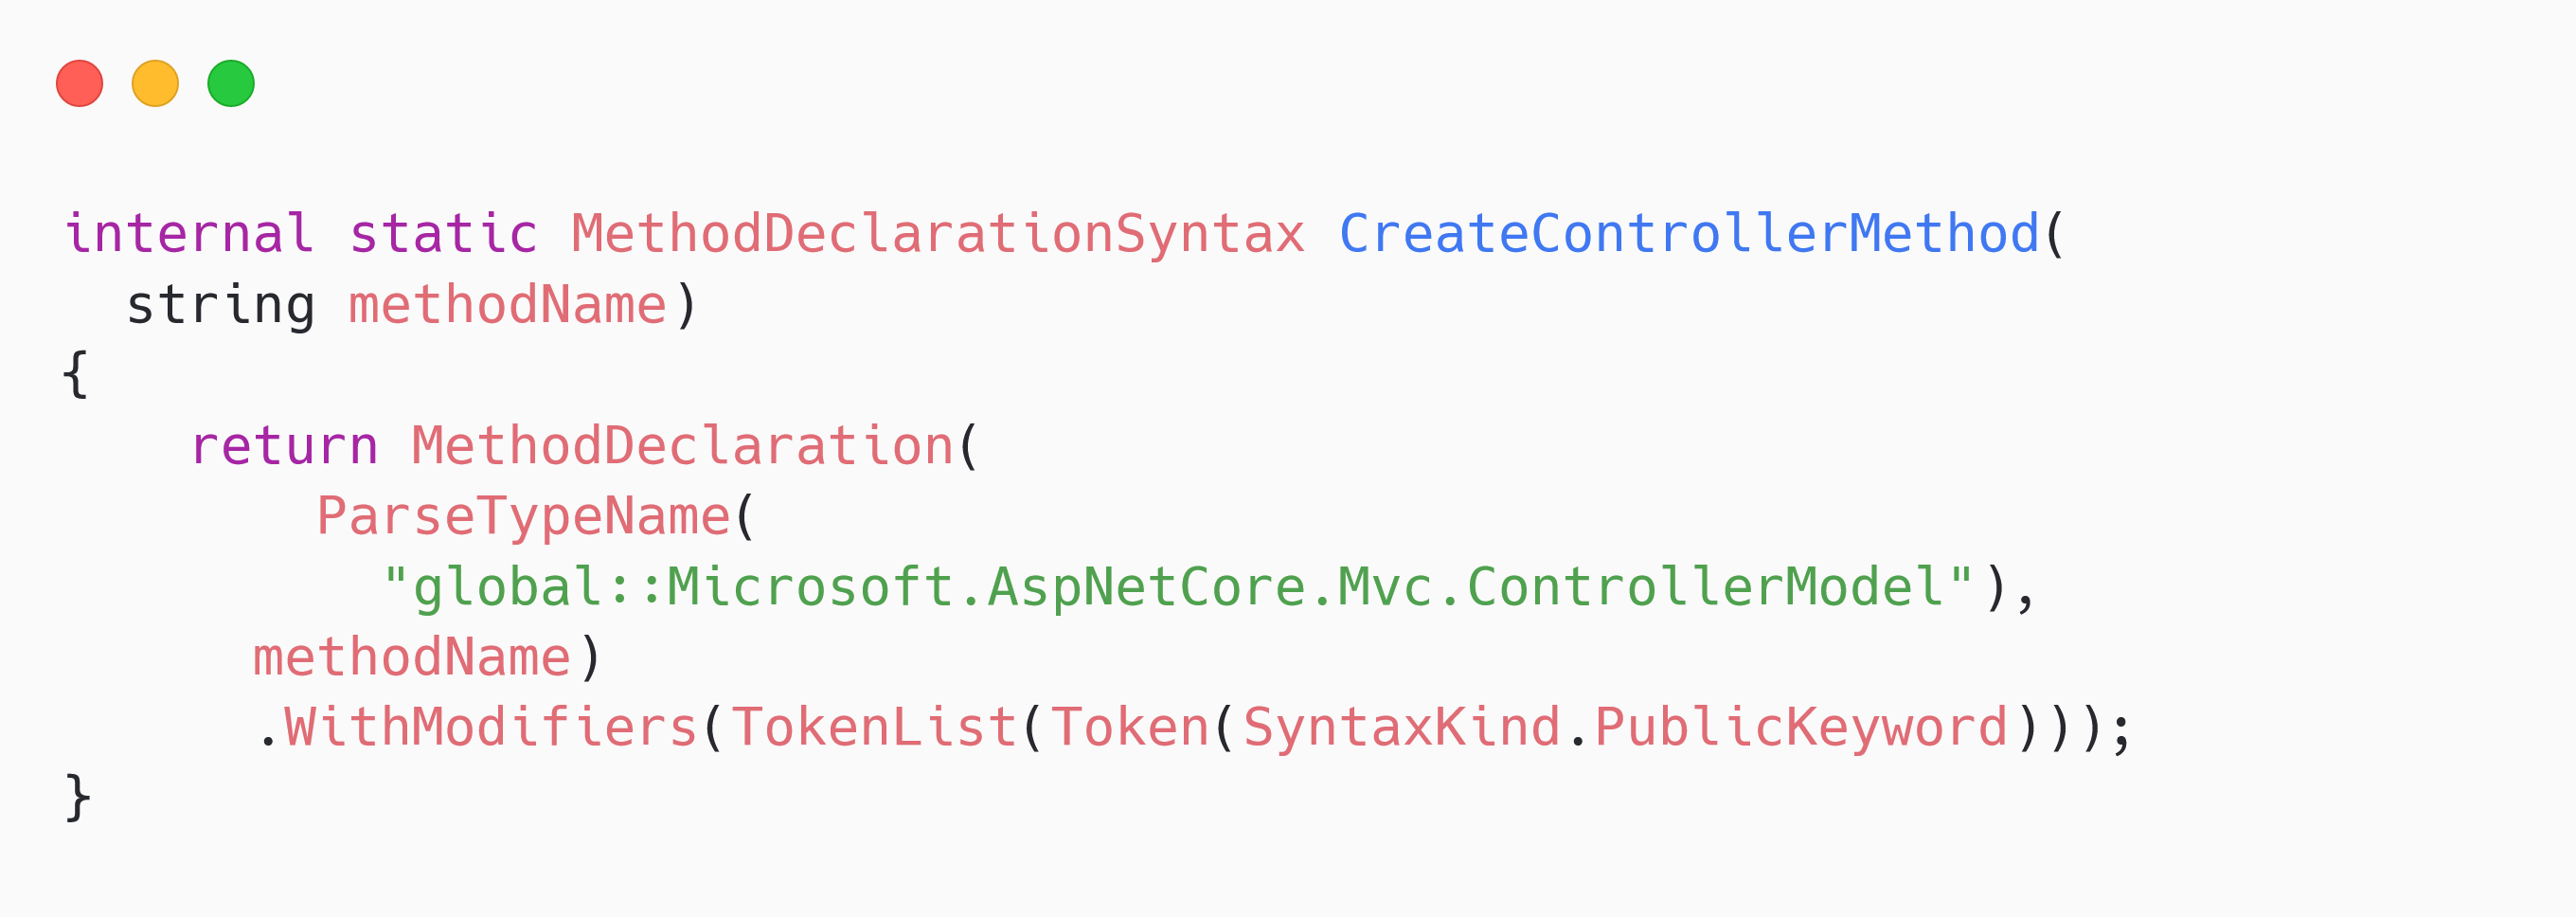
\includegraphics[width=0.8\textwidth]{graphics/syntax-factory.png}
\caption{An example of using SyntaxFactory to generate source code}
\label{fig:syntax-factory}
\end{figure}

\section{Performance Metrics and Evaluation}

To answer our research question— "How does using C\# source generators to convert reflective routing operations into static code in ASP.NET Core impact runtime performance, memory usage, and build time duration?"—we need an accurate way of benchmarking the dynamic and static action discovery test applications. The ultimate goal is to determine if static action discovery is a viable approach to reduce the startup time of ASP.NET Core applications and understand the impact of static action discovery on build time and memory usage. We anticipate a significant improvement in startup speed, even usage of memory, and a slight increase in build duration.

\subsection{Choice of Metrics}

In our quest to determine the impact of using C\# source generators to convert reflective routing operations into static code in ASP.NET Core, three pivotal metrics were chosen—startup duration, build time, and memory usage during startup. The selection of these metrics was driven by the ultimate aim of enhancing operational efficiency in enterprise environments, particularly within the realm of cloud deployments.

The speed at which an application starts up holds paramount importance in contexts like serverless architectures, where applications are frequently spun up and shut down. Consequently, startup duration was selected as one of our primary metrics. An expedited startup process could notably decrease operational costs and foster scalability, two objectives that are crucial for enterprise companies striving to improve their workflows.

Our second metric, build time, was chosen to ensure that the introduction of static action discovery does not excessively impede developer productivity. Lengthy build times could potentially slow down the development process, posing challenges, especially in agile development environments that rely on rapid iteration cycles. Moreover, in the context of continuous integration / continuous deployment (CI/CD) scenarios, protracted build times could delay the deployment of updates and fixes, adversely affecting the flexibility and velocity of a team's development operations.

Lastly, we chose to monitor memory usage during startup. In real-world systems, memory is a finite and valuable resource that is integral to application performance. Excessive memory usage can induce a variety of adverse effects. It can retard the startup process, as the system might need to allocate and deallocate memory. It could also strain the performance of other applications sharing the same system due to the heightened pressure on the system's memory resources. In cloud-based environments, where applications are billed based on their resource consumption, high memory usage can inflate operational costs. Moreover, applications that require less memory are generally easier to scale and distribute across various instances.

We also contemplated other metrics, such as Request Handling Time, CPU Usage, and Request Throughput. However, these were ultimately dismissed from our selection as they would remain unaffected by our approach. After the application has started, the produced Application Model, containing all the information required by the routing mechanism, remains identical whether it is produced by the dynamic or the static action discovery. The sole difference lies in how the Application Model is constructed; its subsequent usage remains constant. With respect to CPU Usage, we concluded that Startup Speed provided a more comprehensive gauge of the startup performance of the two benchmark applications.

\subsection{Benchmarking the Action Discovery}

Defining startup duration requires careful consideration. While the most straightforward approach might be to time the execution of the main function of our application, this approach proves inadequate. The main function is shown in Figure \ref{fig:startup-method}.

\begin{figure}[H]
\centering
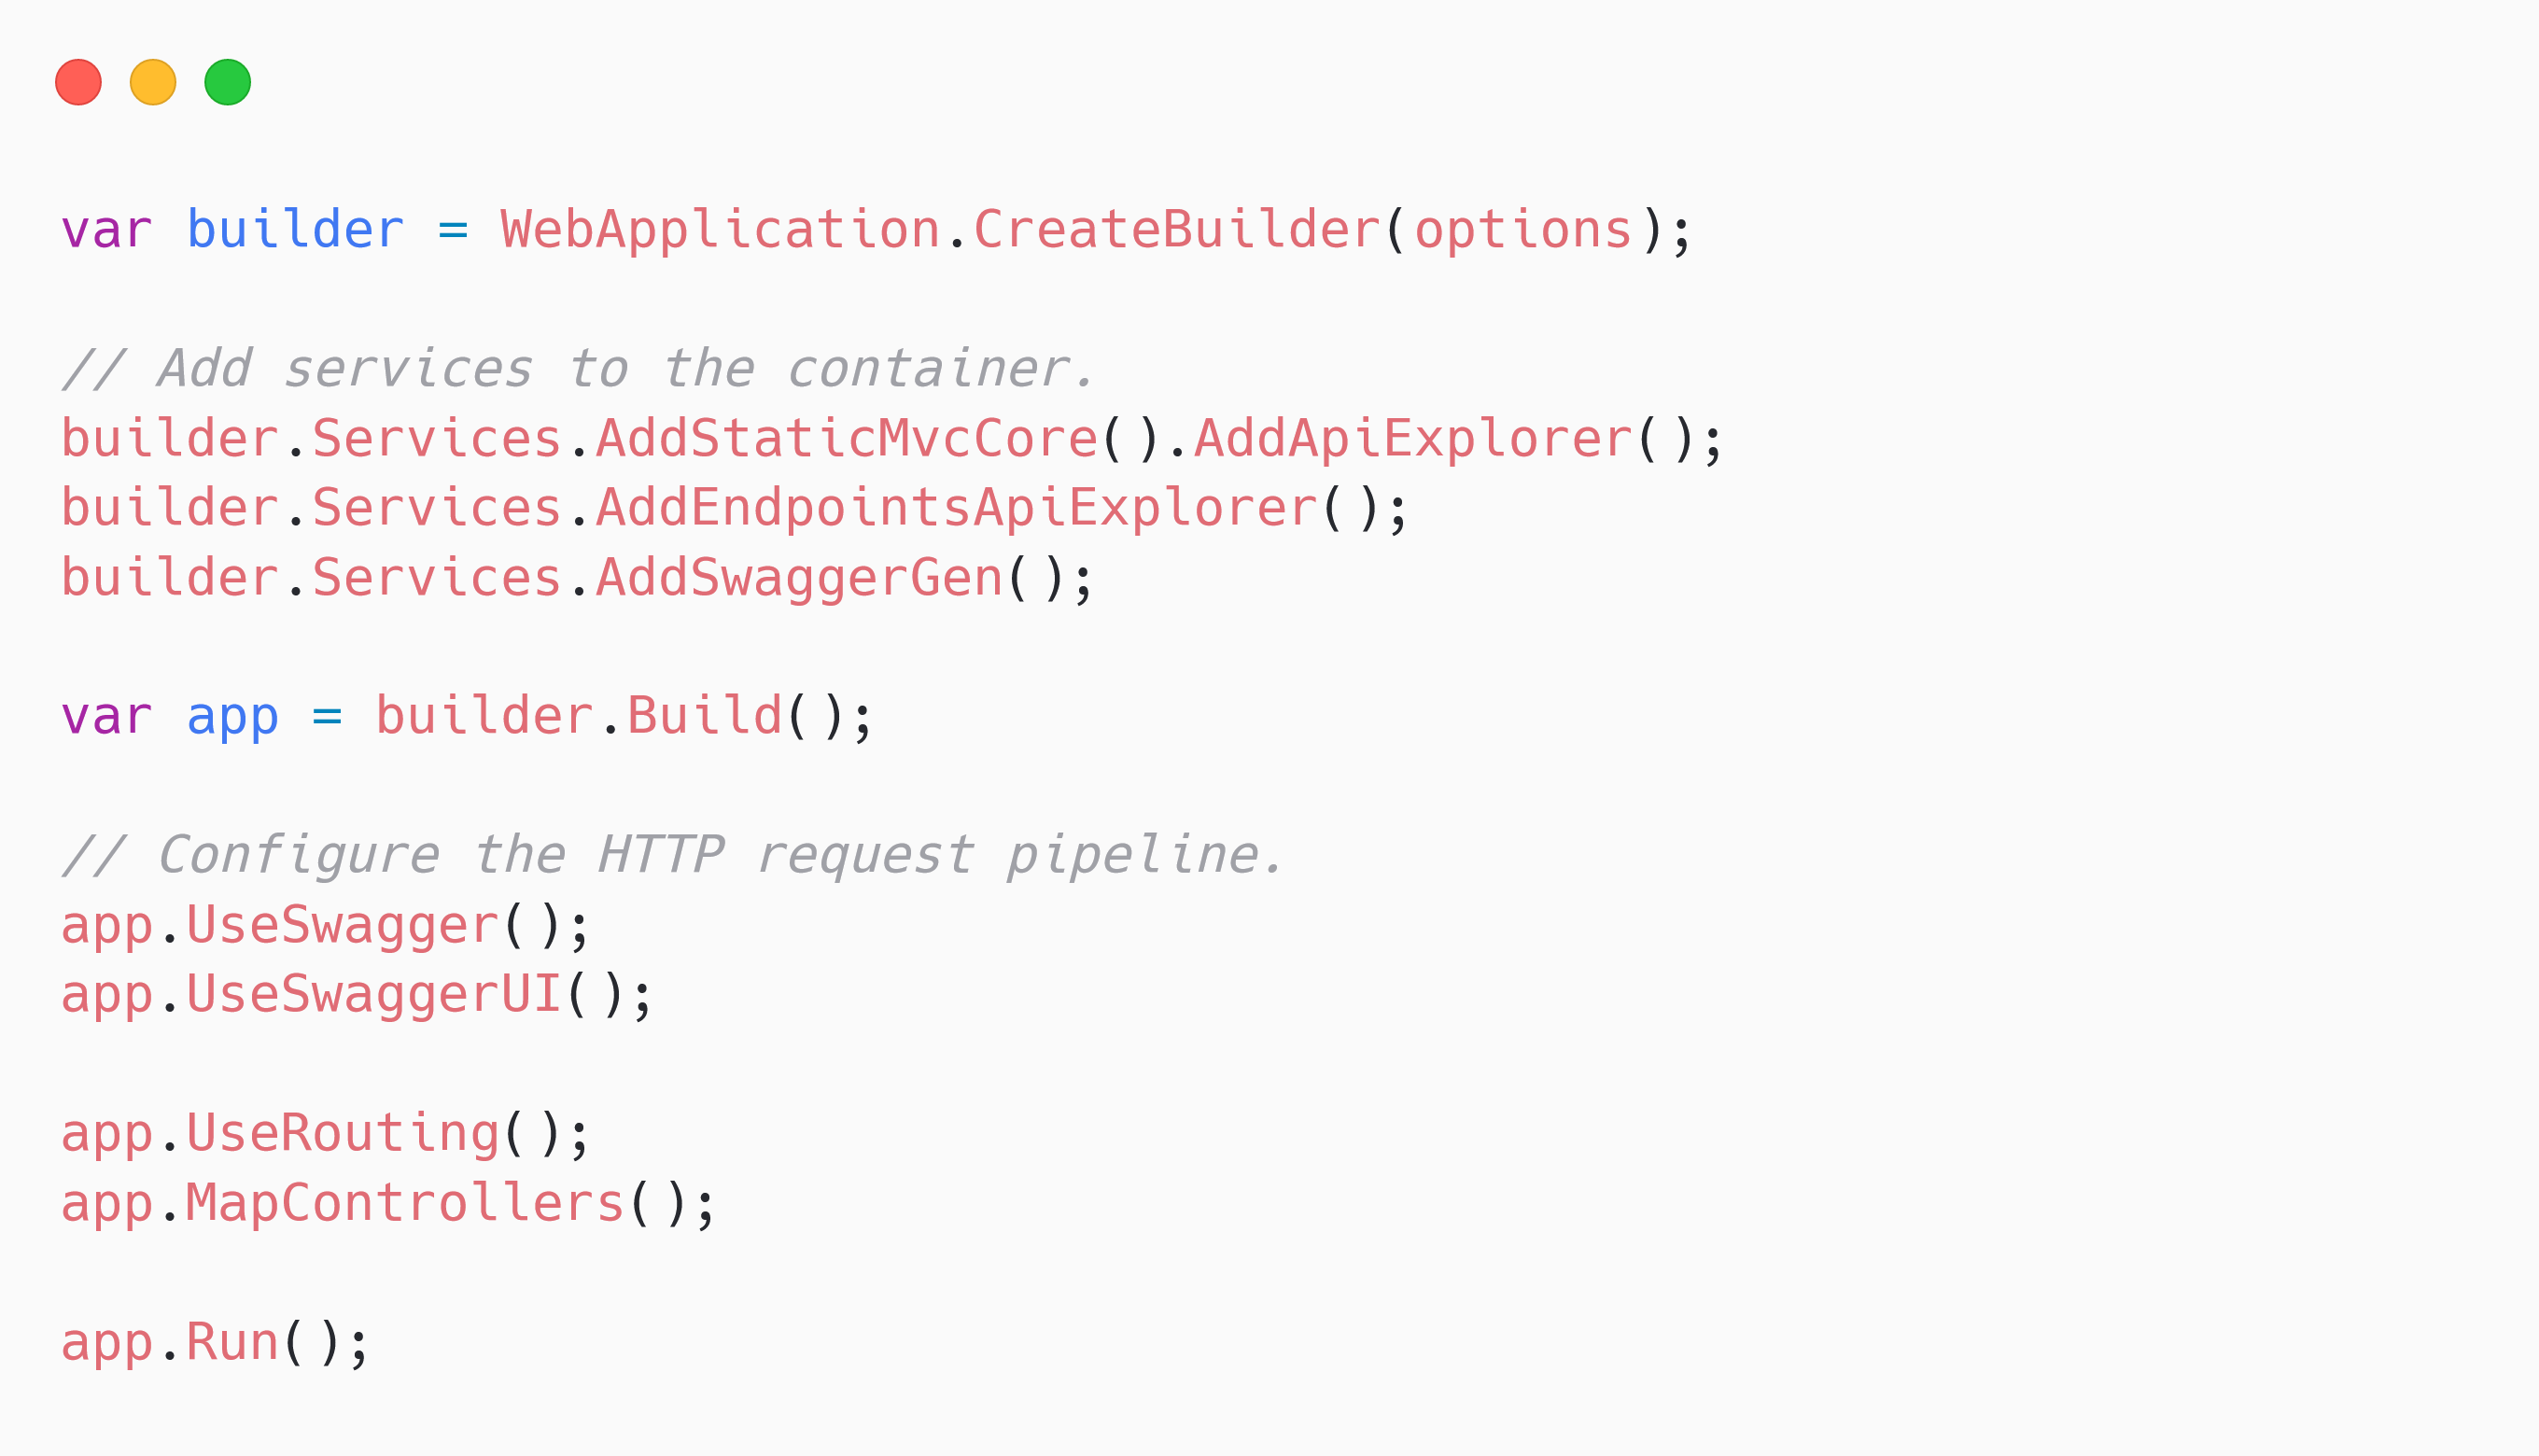
\includegraphics[width=0.8\textwidth]{graphics/startup-method.png}
\caption{The main function of the application, responsible for initializing and running the web server}
\label{fig:startup-method}
\end{figure}

The reason for this lies in the functionality of the "app.Run()" method in the code, which initiates a loop for the web application that only concludes once the application shuts down.

Another alternative could be to time the execution of the MapControllers() method since it performs the action discovery. However, this method does not accurately represent the total startup time of the application.

To navigate these complications, we opt to capture the "ServerReady" log message, which app.Run() logs when the server is ready to receive user requests. Thus, the startup time is defined as the duration from the start of the main method execution until the "ServerReady" log message is logged.

In terms of the methodology for measuring time and memory, the initial thought might be to use a Stopwatch provided by the .NET framework. The Stopwatch would start before the main function execution and stop when the "ServerReady" message is received. However, to ensure the reliability of the results, one would need to execute several warm-up iterations until the benchmark achieves a steady state, perform the main iterations multiple times, and then calculate the necessary statistics.

Given these considerations, it's more efficient to use a dedicated framework. Several such frameworks are available in .NET, including BenchmarkDotNet, NBench, MiniProfiler, and Perfolizer. Based on popularity, as gauged by GitHub, and the fact that Microsoft uses it for benchmarking in the official ASP.NET Core repository, we choose BenchmarkDotNet. Furthermore, BenchmarkDotNet allows us to measure allocated heap memory, which is used to evaluate memory usage during startup.

Finally, measuring build time is executed using the official MSBuild tool, Microsoft's compiler. However, this task is not as simple as it might seem. The project is housed within the official ASP.NET Core repository, which contains over 550 projects. To acquire meaningful results, we compile all dependent projects before measuring the build time and instruct the build tool to only compile the target benchmark application.

The measurement of build time also needs to be conducted multiple times to ensure the results are meaningful. The build results are cached after every build, which can drastically alter build times after the initial build. Therefore, we ensure that all artifacts related only to the project, and not its dependencies, are cleared between builds. As the build time is designed to assess the impact on release workflow, we use the Release configuration for the builds. Since the compiler doesn't provide a build duration, we use the PowerShell Measure-Command tool to gauge the compiler's processing time.

\subsection{Procedure and Methodology for Evaluating Startup Time, Build Time, and Memory Usage}

Assessing three metrics - startup time, build time, and memory usage during startup - requires careful planning to make sure the results are as useful as possible. In each trial, we either run a benchmark with BenchmarkDotNet 200 times or measure the project's compilation time 100 times. We chose these numbers to get a big enough dataset for trustworthy statistical analysis, which helps to lessen the effect of outliers and makes patterns easier to spot.

Starting an ASP.NET web server involves activating many services and executing different classes. Because of this, there are a lot of variables that can interfere with the results. These include Just-In-Time (JIT) compilation, CPUs warming up because modern CPUs can change their frequency based on workload to save energy, and CPU caching, where CPUs can store frequently used data in lower cache levels for faster access.

To minimize these variables' influence and ensure the results are meaningful, we run each benchmark four times. After these runs, we calculate statistics based on the combined results of all four runs. Since the build time isn't affected as much by these variables, as there is no JIT involved, we don't repeat this process for it. The higher variance of the results is also the reason why the benchmark trials contain twice the amount of runs as the compilation trials.

Trials are conducted using a specific setup to ensure consistent and reliable results. The machine used for these trials is rebooted after each run to ensure minimal background tasks are running, thus preventing any interference with the results. Each reboot clears potential residual tasks from the previous trial, providing a clean state for the next one. This methodology is instrumental in ensuring that no other applications interfere with the benchmarking process.

Table \ref{table:specifications} provides an overview of the software and hardware specifications used throughout the trials, which includes information about the operating system, CPU, BenchmarkDotNet version, and .NET version. This setup is consistently maintained to ensure the integrity and consistency of the benchmarking process. As the project is part of the official ASP.NET Core repository, it has access to the latest .NET SDK, enabling trials to be performed using the most recent versions.

Using the latest versions helps ensure that the project benefits from the most recent advancements and optimizations in the software, contributing to the relevance and applicability of the results. The trials can robustly assess the solution's performance across different scenarios by specifying and controlling these factors.

\begin{table}[h!]
\centering
\begin{tabular}{|c|c|}
\hline
\textbf{Component} & \textbf{Version} \\
\hline
Operating System & Windows 11 (Build: 22621.1848) \\
\hline
CPU & 13th Gen Intel Core i9-13900K \\
\hline
BenchmarkDotNet Version & 0.13.0 \\
\hline
.NET Version & 8.0.100 preview 5 \\
\hline
\end{tabular}
\caption{Machine and Software Specifications for the Trials}
\label{table:specifications}
\end{table}

Mean values, error, and standard deviation are recorded for each of the 100 runs during a trial. Here, 'error' refers to half of the 99.9\% confidence interval. A 99.9\% confidence interval means there is a 99.9\% probability that the interval contains the true population mean. The 'half' is taken to provide a margin of error, which is a range where the true value lies with a certain level of confidence. This data is visualized to simplify interpretation and facilitate comparison between static and dynamic action discovery benchmarks.

Trials are carried out on projects of varying sizes to assess the scalability of the solution and its performance under different scenarios. It starts with a small application of 100 Controllers to establish a baseline, followed by a medium-sized application of 1000 Controllers, and finally, an enterprise-scale application with 10,000 Controllers. It's worth noting that only the number of controllers varies for this analysis, while the number of non-controller classes remains constant. The proposed solution is expected to be more efficient in projects where there are more non-controller classes, as dynamic action discovery needs to analyze these classes on every startup, whereas static action discovery does not, as it generates no code for non-controller classes. However, the focus here remains on applications with varying controller sizes to isolate the impact of this single variable on the results.

Once the trials are complete, results from static and dynamic action discovery benchmarks are compared to identify significant differences. This process is designed to generate raw data and uncover meaningful insights that can guide future improvements in the action discovery process.

It is important to remember that every analysis has potential biases or limitations, and these are considered carefully when interpreting the data. The benchmarks are conducted under specific conditions, and results may differ with different configurations or workloads. Any assumptions made during the analysis are transparently communicated. This rigor ensures the most accurate interpretation and valuable conclusions.
